
\setcounter{chapter}{0} 

%% IMPORTANT:   from this file, refer to the bibliography as   Neutrino/NF01/bibliography.tex   
%%    refer to a figure   A.pdf  as    Neutrino/NF01/figures/A.pdf  .

\chapter{Neutrino Oscillations}

\authorlist{P. B. Denton, M. Friend, M. Messier, H. Tanaka}
   {(contributors from the community)}


Already we are boldly launched upon the deep; but soon we shall be lost in its unshored, harbourless immensities. Ere that come to pass; ere the Pequod’s weedy hull rolls side by side with the barnacled hulls of the leviathan; at the outset it is but well to attend to a matter almost indispensable to a thorough appreciative understanding of the more special leviathanic revelations and allusions of all sorts which are to follow.

It is some systematized exhibition of the whale in his broad genera, that I would now fain put before you. Yet is it no easy task. The classification of the constituents of a chaos, nothing less is here essayed. Listen to what the best and latest authorities have laid down.

``No branch of Zoology is so much involved as that which is entitled Cetology,'' says Captain Scoresby, A.D. 1820~\cite{N1-Scoresby}.

``It is not my intention, were it in my power, to enter into the inquiry as to the true method of dividing the cetacea into groups and families. $\cdots$ Utter confusion exists among the historians of this animal'' (sperm whale), says Surgeon Beale, A.D. 1839~\cite{N1-Beale}.

``Unfitness to pursue our research in the unfathomable waters.'' ``Impenetrable veil covering our knowledge of the cetacea.''  ``A field strewn with thorns.'' ``All these incomplete indications but serve to torture us naturalists.''~\cite{N1-Cuvier,N1-Hunter,N1-Lesson}

Thus speak of the whale, the great Cuvier, and John Hunter, and Lesson, those lights of zoology and anatomy. Nevertheless, though of real knowledge there be little, yet of books there are a plenty; and so in some small degree, with cetology, or the science of whales. Many are the men, small and great, old and new, landsmen and seamen, who have at large or in little, written of the whale. Run over a few: The Authors of the Bible; Aristotle; Pliny; Aldrovandi; Sir Thomas Browne; Gesner; Ray; Linnæus; Rondeletius; Willoughby; Green; Artedi; Sibbald; Brisson; Marten; Lacépède; Bonneterre; Desmarest; Baron Cuvier; Frederick Cuvier; John Hunter; Owen; Scoresby; Beale; Bennett; J. Ross Browne; the Author of Miriam Coffin; Olmstead; and the Rev. T. Cheever. But to what ultimate generalizing purpose all these have written, the above cited extracts will show.

Of the names in this list of whale authors, only those following Owen ever saw living whales; and but one of them was a real professional harpooneer and whaleman. I mean Captain Scoresby. On the separate subject of the Greenland or right-whale, he is the best existing authority. But Scoresby knew nothing and says nothing of the great sperm whale, compared with which the Greenland whale is almost unworthy mentioning. And here be it said, that the Greenland whale is an usurper upon the throne of the seas. He is not even by any means the largest of the whales. Yet, owing to the long priority of his claims, and the profound ignorance which, till some seventy years back, invested the then fabulous or utterly unknown sperm-whale, and which ignorance to this present day still reigns in all but some few scientific retreats and whale-ports; this usurpation has been every way complete. Reference to nearly all the leviathanic allusions in the great poets of past days, will satisfy you that the Greenland whale, without one rival, was to them the monarch of the seas. But the time has at last come for a new proclamation. This is Charing Cross; hear ye! good people all,---the Greenland whale is deposed,---the great sperm whale now reigneth!

There are only two books in being which at all pretend to put the living sperm whale before you, and at the same time, in the remotest degree succeed in the attempt. Those books are Beale’s and Bennett’s; both in their time surgeons to English South-Sea whale-ships, and both exact and reliable men. The original matter touching the sperm whale to be found in their volumes is necessarily small; but so far as it goes, it is of excellent quality, though mostly confined to scientific description. As yet, however, the sperm whale, scientific or poetic, lives not complete in any literature. Far above all other hunted whales, his is an unwritten life.

Now the various species of whales need some sort of popular comprehensive classification, if only an easy outline one for the present, hereafter to be filled in all its departments by subsequent laborers. As no better man advances to take this matter in hand, I hereupon offer my own poor endeavors. I promise nothing complete; because any human thing supposed to be complete, must for that very reason infallibly be faulty. I shall not pretend to a minute anatomical description of the various species, or---in this place at least—to much of any description. My object here is simply to project the draught of a systematization of cetology. I am the architect, not the builder.

But it is a ponderous task; no ordinary letter-sorter in the Post-Office is equal to it. To grope down into the bottom of the sea after them; to have one’s hands among the unspeakable foundations, ribs, and very pelvis of the world; this is a fearful thing. What am I that I should essay to hook the nose of this leviathan! The awful tauntings in Job might well appal me. Will he (the leviathan) make a covenant with thee? Behold the hope of him is vain! But I have swam through libraries and sailed through oceans; I have had to do with whales with these visible hands; I am in earnest; and I will try. There are some preliminaries to settle.

First: The uncertain, unsettled condition of this science of Cetology is in the very vestibule attested by the fact, that in some quarters it still remains a moot point whether a whale be a fish. In his System of Nature, A.D. 1776, Linnæus declares, “I hereby separate the whales from the fish.” But of my own knowledge, I know that down to the year 1850, sharks and shad, alewives and herring, against Linnæus’s express edict, were still found dividing the possession of the same seas with the Leviathan.

The grounds upon which Linnæus would fain have banished the whales from the waters, he states as follows: “On account of their warm bilocular heart, their lungs, their movable eyelids, their hollow ears, penem intrantem feminam mammis lactantem,” and finally, “ex lege naturæ jure meritoque.” I submitted all this to my friends Simeon Macey and Charley Coffin, of Nantucket, both messmates of mine in a certain voyage, and they united in the opinion that the reasons set forth were altogether insufficient. Charley profanely hinted they were humbug.

Be it known that, waiving all argument, I take the good old fashioned ground that the whale is a fish, and call upon holy Jonah to back me. This fundamental thing settled, the next point is, in what internal respect does the whale differ from other fish. Above, Linnæus has given you those items. But in brief, they are these: lungs and warm blood; whereas, all other fish are lungless and cold blooded.

Next: how shall we define the whale, by his obvious externals, so as conspicuously to label him for all time to come? To be short, then, a whale is a spouting fish with a horizontal tail. There you have him. However contracted, that definition is the result of expanded meditation. A walrus spouts much like a whale, but the walrus is not a fish, because he is amphibious. But the last term of the definition is still more cogent, as coupled with the first. Almost any one must have noticed that all the fish familiar to landsmen have not a flat, but a vertical, or up-and-down tail. Whereas, among spouting fish the tail, though it may be similarly shaped, invariably assumes a horizontal position.

By the above definition of what a whale is, I do by no means exclude from the leviathanic brotherhood any sea creature hitherto identified with the whale by the best informed Nantucketers; nor, on the other hand, link with it any fish hitherto authoritatively regarded as alien~\footnote{I am aware that down to the present time, the fish styled Lamatins and Dugongs (Pig-fish and Sow-fish of the Coffins of Nantucket) are included by many naturalists among the whales. But as these pig-fish are a noisy, contemptible set, mostly lurking in the mouths of rivers, and feeding on wet hay, and especially as they do not spout, I deny their credentials as whales; and have presented them with their passports to quit the Kingdom of Cetology.} Hence, all the smaller, spouting, and horizontal tailed fish must be included in this ground-plan of Cetology. Now, then, come the grand divisions of the entire whale host.

%%%%%%%%%%%%%%%%%%%%%%%%%%%%%%%%%%%%%%%%%%%%%%%%%%%%%%%%%%%%%%%%%%%%%%%%%
\begin{figure}
\begin{center}
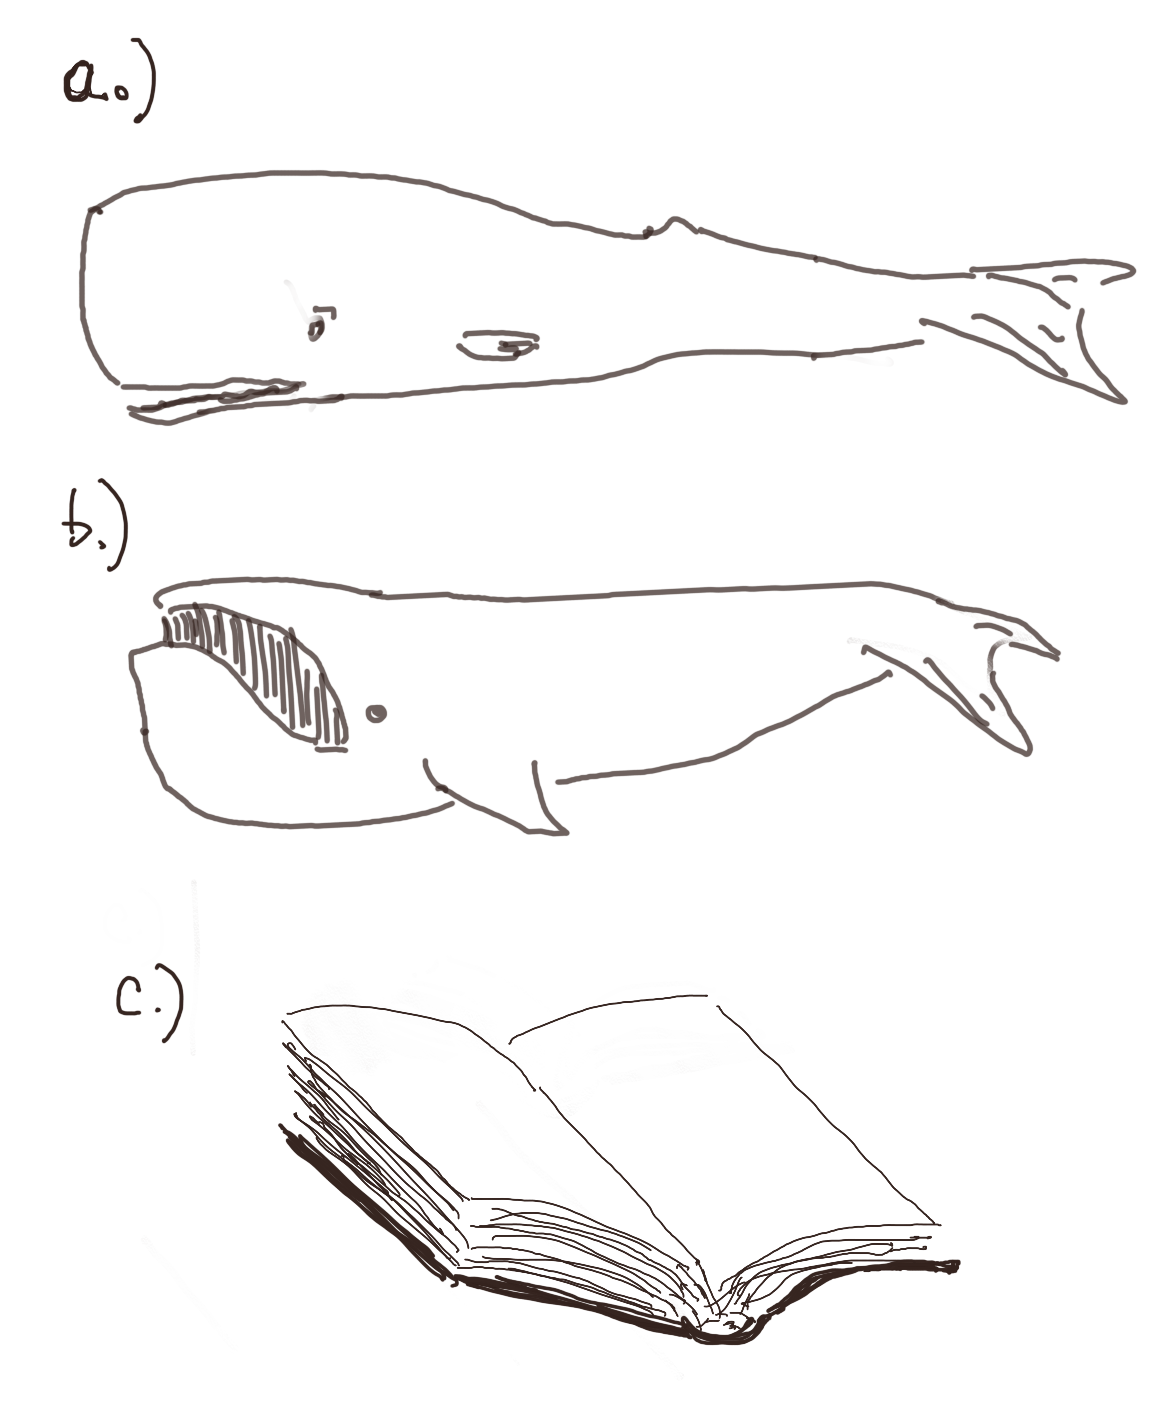
\includegraphics[width=0.40\hsize]{Neutrino/NF01/figures/Whales.png}
\end{center}
\caption{(a) Sperm Whale (b) Right Whale, (c) ``$\ldots$, or, The Whale''.}
\label{fig:NF1-Whale}
\end{figure}
%%%%%%%%%%%%%%%%%%%%%%%%%%%%%%%%%%%%%%%%%%%%%%%%%%%%%%%%%%%%%%%%%%%%%%%%%%%

First: According to magnitude I divide the whales into three primary BOOKS (subdivisible into CHAPTERS), and these shall comprehend them all, both small and large.

I. THE FOLIO WHALE; II. the OCTAVO WHALE; III. the DUODECIMO WHALE.

As the type of the FOLIO I present the Sperm Whale; of the OCTAVO, the Grampus; of the DUODECIMO, the Porpoise.

\section{Folio}

FOLIOS. Among these I here include the following chapters:—I. The Sperm Whale; II. the Right Whale; III. the Fin-Back Whale; IV. the Hump-backed Whale; V. the Razor Back Whale; VI. the Sulphur Bottom Whale.
(See Fig.~\ref{fig:NF1-Whale}.)

\subsection{Sperm Whale}

BOOK I. (Folio), CHAPTER I. (Sperm Whale).—This whale, among the English of old vaguely known as the Trumpa whale, and the Physeter whale, and the Anvil Headed whale, is the present Cachalot of the French, and the Pottsfich of the Germans, and the Macrocephalus of the Long Words. He is, without doubt, the largest inhabitant of the globe; the most formidable of all whales to encounter; the most majestic in aspect; and lastly, by far the most valuable in commerce; he being the only creature from which that valuable substance, spermaceti, is obtained. All his peculiarities will, in many other places, be enlarged upon. It is chiefly with his name that I now have to do. Philologically considered, it is absurd. Some centuries ago, when the Sperm whale was almost wholly unknown in his own proper individuality, and when his oil was only accidentally obtained from the stranded fish; in those days spermaceti, it would seem, was popularly supposed to be derived from a creature identical with the one then known in England as the Greenland or Right Whale. It was the idea also, that this same spermaceti was that quickening humor of the Greenland Whale which the first syllable of the word literally expresses. In those times, also, spermaceti was exceedingly scarce, not being used for light, but only as an ointment and medicament. It was only to be had from the druggists as you nowadays buy an ounce of rhubarb. When, as I opine, in the course of time, the true nature of spermaceti became known, its original name was still retained by the dealers; no doubt to enhance its value by a notion so strangely significant of its scarcity. And so the appellation must at last have come to be bestowed upon the whale from which this spermaceti was really derived.

\subsection{Right Whale}

BOOK I. (Folio), CHAPTER II. (Right Whale).—In one respect this is the most venerable of the leviathans, being the one first regularly hunted by man. It yields the article commonly known as whalebone or baleen; and the oil specially known as “whale oil,” an inferior article in commerce. Among the fishermen, he is indiscriminately designated by all the following titles: The Whale; the Greenland Whale; the Black Whale; the Great Whale; the True Whale; the Right Whale. There is a deal of obscurity concerning the identity of the species thus multitudinously baptised. What then is the whale, which I include in the second species of my Folios? It is the Great Mysticetus of the English naturalists; the Greenland Whale of the English whalemen; the Baleine Ordinaire of the French whalemen; the Growlands Walfish of the Swedes. It is the whale which for more than two centuries past has been hunted by the Dutch and English in the Arctic seas; it is the whale which the American fishermen have long pursued in the Indian ocean, on the Brazil Banks, on the Nor’ West Coast, and various other parts of the world, designated by them Right Whale Cruising Grounds.

Some pretend to see a difference between the Greenland whale of the English and the right whale of the Americans. But they precisely agree in all their grand features; nor has there yet been presented a single determinate fact upon which to ground a radical distinction. It is by endless subdivisions based upon the most inconclusive differences, that some departments of natural history become so repellingly intricate. The right whale will be elsewhere treated of at some length, with reference to elucidating the sperm whale.

\subsection{Fin-Back Whale}

BOOK I. (Folio), CHAPTER III. (Fin-Back).—Under this head I reckon a monster which, by the various names of Fin-Back, Tall-Spout, and Long-John, has been seen almost in every sea and is commonly the whale whose distant jet is so often descried by passengers crossing the Atlantic, in the New York packet-tracks. In the length he attains, and in his baleen, the Fin-back resembles the right whale, but is of a less portly girth, and a lighter colour, approaching to olive. His great lips present a cable-like aspect, formed by the intertwisting, slanting folds of large wrinkles. His grand distinguishing feature, the fin, from which he derives his name, is often a conspicuous object. This fin is some three or four feet long, growing vertically from the hinder part of the back, of an angular shape, and with a very sharp pointed end. Even if not the slightest other part of the creature be visible, this isolated fin will, at times, be seen plainly projecting from the surface. When the sea is moderately calm, and slightly marked with spherical ripples, and this gnomon-like fin stands up and casts shadows upon the wrinkled surface, it may well be supposed that the watery circle surrounding it somewhat resembles a dial, with its style and wavy hour-lines graved on it. On that Ahaz-dial the shadow often goes back. The Fin-Back is not gregarious. He seems a whale-hater, as some men are man-haters. Very shy; always going solitary; unexpectedly rising to the surface in the remotest and most sullen waters; his straight and single lofty jet rising like a tall misanthropic spear upon a barren plain; gifted with such wondrous power and velocity in swimming, as to defy all present pursuit from man; this leviathan seems the banished and unconquerable Cain of his race, bearing for his mark that style upon his back. From having the baleen in his mouth, the Fin-Back is sometimes included with the right whale, among a theoretic species denominated Whalebone whales, that is, whales with baleen. Of these so called Whalebone whales, there would seem to be several varieties, most of which, however, are little known. Broad-nosed whales and beaked whales; pike-headed whales; bunched whales; under-jawed whales and rostrated whales, are the fishermen’s names for a few sorts.

In connection with this appellative of ``Whalebone whales'', it is of great importance to mention, that however such a nomenclature may be convenient in facilitating allusions to some kind of whales, yet it is in vain to attempt a clear classification of the Leviathan, founded upon either his baleen, or hump, or fin, or teeth; notwithstanding that those marked parts or features very obviously seem better adapted to afford the basis for a regular system of Cetology than any other detached bodily distinctions, which the whale, in his kinds, presents. How then? The baleen, hump, back-fin, and teeth; these are things whose peculiarities are indiscriminately dispersed among all sorts of whales, without any regard to what may be the nature of their structure in other and more essential particulars. Thus, the sperm whale and the humpbacked whale, each has a hump; but there the similitude ceases. Then, this same humpbacked whale and the Greenland whale, each of these has baleen; but there again the similitude ceases. And it is just the same with the other parts above mentioned. In various sorts of whales, they form such irregular combinations; or, in the case of any one of them detached, such an irregular isolation; as utterly to defy all general methodization formed upon such a basis. On this rock every one of the whale-naturalists has split.

But it may possibly be conceived that, in the internal parts of the whale, in his anatomy—there, at least, we shall be able to hit the right classification. Nay; what thing, for example, is there in the Greenland whale’s anatomy more striking than his baleen? Yet we have seen that by his baleen it is impossible correctly to classify the Greenland whale. And if you descend into the bowels of the various leviathans, why there you will not find distinctions a fiftieth part as available to the systematizer as those external ones already enumerated. What then remains? nothing but to take hold of the whales bodily, in their entire liberal volume, and boldly sort them that way. And this is the Bibliographical system here adopted; and it is the only one that can possibly succeed, for it alone is practicable. To proceed.

\subsection{Hump Back Whale}

BOOK I. (Folio) CHAPTER IV. (Hump Back).—This whale is often seen on the northern American coast. He has been frequently captured there, and towed into harbor. He has a great pack on him like a peddler; or you might call him the Elephant and Castle whale. At any rate, the popular name for him does not sufficiently distinguish him, since the sperm whale also has a hump though a smaller one. His oil is not very valuable. He has baleen. He is the most gamesome and light-hearted of all the whales, making more gay foam and white water generally than any other of them.

\subsection{Razor Back Whale}

BOOK I. (Folio), CHAPTER V. (Razor Back).—Of this whale little is known but his name. I have seen him at a distance off Cape Horn. Of a retiring nature, he eludes both hunters and philosophers. Though no coward, he has never yet shown any part of him but his back, which rises in a long sharp ridge. Let him go. I know little more of him, nor does anybody else.

\subsection{Sulpher Bottom Whale}

BOOK I. (Folio), CHAPTER VI. (Sulphur Bottom).—Another retiring gentleman, with a brimstone belly, doubtless got by scraping along the Tartarian tiles in some of his profounder divings. He is seldom seen; at least I have never seen him except in the remoter southern seas, and then always at too great a distance to study his countenance. He is never chased; he would run away with rope-walks of line. Prodigies are told of him. Adieu, Sulphur Bottom! I can say nothing more that is true of ye, nor can the oldest Nantucketer.

Thus ends BOOK I. (Folio), and now begins BOOK II. (Octavo).

\section{Octavo}

OCTAVOES.*—These embrace the whales of middling magnitude, among which present may be numbered:—I., the Grampus; II., the Black Fish; III., the Narwhale; IV., the Thrasher; V., the Killer.

*Why this book of whales is not denominated the Quarto is very plain. Because, while the whales of this order, though smaller than those of the former order, nevertheless retain a proportionate likeness to them in figure, yet the bookbinder’s Quarto volume in its dimensioned form does not preserve the shape of the Folio volume, but the Octavo volume does.

\subsection{Grampus}

BOOK II. (Octavo), CHAPTER I. (Grampus).—Though this fish, whose loud sonorous breathing, or rather blowing, has furnished a proverb to landsmen, is so well known a denizen of the deep, yet is he not popularly classed among whales. But possessing all the grand distinctive features of the leviathan, most naturalists have recognised him for one. He is of moderate octavo size, varying from fifteen to twenty-five feet in length, and of corresponding dimensions round the waist. He swims in herds; he is never regularly hunted, though his oil is considerable in quantity, and pretty good for light. By some fishermen his approach is regarded as premonitory of the advance of the great sperm whale.

\subsection{Black Fish}

BOOK II. (Octavo), CHAPTER II. (Black Fish).—I give the popular fishermen’s names for all these fish, for generally they are the best. Where any name happens to be vague or inexpressive, I shall say so, and suggest another. I do so now, touching the Black Fish, so-called, because blackness is the rule among almost all whales. So, call him the Hyena Whale, if you please. His voracity is well known, and from the circumstance that the inner angles of his lips are curved upwards, he carries an everlasting Mephistophelean grin on his face. This whale averages some sixteen or eighteen feet in length. He is found in almost all latitudes. He has a peculiar way of showing his dorsal hooked fin in swimming, which looks something like a Roman nose. When not more profitably employed, the sperm whale hunters sometimes capture the Hyena whale, to keep up the supply of cheap oil for domestic employment—as some frugal housekeepers, in the absence of company, and quite alone by themselves, burn unsavory tallow instead of odorous wax. Though their blubber is very thin, some of these whales will yield you upwards of thirty gallons of oil.

\subsection{Narwhale}

BOOK II. (Octavo), CHAPTER III. (Narwhale), that is, Nostril whale.—Another instance of a curiously named whale, so named I suppose from his peculiar horn being originally mistaken for a peaked nose. The creature is some sixteen feet in length, while its horn averages five feet, though some exceed ten, and even attain to fifteen feet. Strictly speaking, this horn is but a lengthened tusk, growing out from the jaw in a line a little depressed from the horizontal. But it is only found on the sinister side, which has an ill effect, giving its owner something analogous to the aspect of a clumsy left-handed man. What precise purpose this ivory horn or lance answers, it would be hard to say. It does not seem to be used like the blade of the sword-fish and bill-fish; though some sailors tell me that the Narwhale employs it for a rake in turning over the bottom of the sea for food. Charley Coffin said it was used for an ice-piercer; for the Narwhale, rising to the surface of the Polar Sea, and finding it sheeted with ice, thrusts his horn up, and so breaks through. But you cannot prove either of these surmises to be correct. My own opinion is, that however this one-sided horn may really be used by the Narwhale—however that may be—it would certainly be very convenient to him for a folder in reading pamphlets. The Narwhale I have heard called the Tusked whale, the Horned whale, and the Unicorn whale. He is certainly a curious example of the Unicornism to be found in almost every kingdom of animated nature. From certain cloistered old authors I have gathered that this same sea-unicorn’s horn was in ancient days regarded as the great antidote against poison, and as such, preparations of it brought immense prices. It was also distilled to a volatile salts for fainting ladies, the same way that the horns of the male deer are manufactured into hartshorn. Originally it was in itself accounted an object of great curiosity. Black Letter tells me that Sir Martin Frobisher on his return from that voyage, when Queen Bess did gallantly wave her jewelled hand to him from a window of Greenwich Palace, as his bold ship sailed down the Thames; “when Sir Martin returned from that voyage,” saith Black Letter, “on bended knees he presented to her highness a prodigious long horn of the Narwhale, which for a long period after hung in the castle at Windsor.” An Irish author avers that the Earl of Leicester, on bended knees, did likewise present to her highness another horn, pertaining to a land beast of the unicorn nature.

The Narwhale has a very picturesque, leopard-like look, being of a milk-white ground colour, dotted with round and oblong spots of black. His oil is very superior, clear and fine; but there is little of it, and he is seldom hunted. He is mostly found in the circumpolar seas.

\subsection{Killer Whale}

BOOK II. (Octavo), CHAPTER IV. (Killer).—Of this whale little is precisely known to the Nantucketer, and nothing at all to the professed naturalist. From what I have seen of him at a distance, I should say that he was about the bigness of a grampus. He is very savage—a sort of Feegee fish. He sometimes takes the great Folio whales by the lip, and hangs there like a leech, till the mighty brute is worried to death. The Killer is never hunted. I never heard what sort of oil he has. Exception might be taken to the name bestowed upon this whale, on the ground of its indistinctness. For we are all killers, on land and on sea; Bonapartes and Sharks included.

\subsection{Thrasher Whale}

BOOK II. (Octavo), CHAPTER V. (Thrasher).—This gentleman is famous for his tail, which he uses for a ferule in thrashing his foes. He mounts the Folio whale’s back, and as he swims, he works his passage by flogging him; as some schoolmasters get along in the world by a similar process. Still less is known of the Thrasher than of the Killer. Both are outlaws, even in the lawless seas.

Thus ends BOOK II. (Octavo), and begins BOOK III. (Duodecimo).

\section{Duodecimo}

DUODECIMOES.—These include the smaller whales. I. The Huzza Porpoise. II. The Algerine Porpoise. III. The Mealy-mouthed Porpoise.

To those who have not chanced specially to study the subject, it may possibly seem strange, that fishes not commonly exceeding four or five feet should be marshalled among WHALES—a word, which, in the popular sense, always conveys an idea of hugeness. But the creatures set down above as Duodecimoes are infallibly whales, by the terms of my definition of what a whale is—i.e. a spouting fish, with a horizontal tail.

\subsection{Huzza Porpoise}

BOOK III. (Duodecimo), CHAPTER 1. (Huzza Porpoise).—This is the common porpoise found almost all over the globe. The name is of my own bestowal; for there are more than one sort of porpoises, and something must be done to distinguish them. I call him thus, because he always swims in hilarious shoals, which upon the broad sea keep tossing themselves to heaven like caps in a Fourth-of-July crowd. Their appearance is generally hailed with delight by the mariner. Full of fine spirits, they invariably come from the breezy billows to windward. They are the lads that always live before the wind. They are accounted a lucky omen. If you yourself can withstand three cheers at beholding these vivacious fish, then heaven help ye; the spirit of godly gamesomeness is not in ye. A well-fed, plump Huzza Porpoise will yield you one good gallon of good oil. But the fine and delicate fluid extracted from his jaws is exceedingly valuable. It is in request among jewellers and watchmakers. Sailors put it on their hones. Porpoise meat is good eating, you know. It may never have occurred to you that a porpoise spouts. Indeed, his spout is so small that it is not very readily discernible. But the next time you have a chance, watch him; and you will then see the great Sperm whale himself in miniature.

\subsection{Algerine Porpoise}

BOOK III. (Duodecimo), CHAPTER II. (Algerine Porpoise).—A pirate. Very savage. He is only found, I think, in the Pacific. He is somewhat larger than the Huzza Porpoise, but much of the same general make. Provoke him, and he will buckle to a shark. I have lowered for him many times, but never yet saw him captured.

\subsection{Mealy-mouthed Porpoise}

BOOK III. (Duodecimo), CHAPTER III. (Mealy-mouthed Porpoise).—The largest kind of Porpoise; and only found in the Pacific, so far as it is known. The only English name, by which he has hitherto been designated, is that of the fishers—Right-Whale Porpoise, from the circumstance that he is chiefly found in the vicinity of that Folio. In shape, he differs in some degree from the Huzza Porpoise, being of a less rotund and jolly girth; indeed, he is of quite a neat and gentleman-like figure. He has no fins on his back (most other porpoises have), he has a lovely tail, and sentimental Indian eyes of a hazel hue. But his mealy-mouth spoils all. Though his entire back down to his side fins is of a deep sable, yet a boundary line, distinct as the mark in a ship’s hull, called the “bright waist,” that line streaks him from stem to stern, with two separate colours, black above and white below. The white comprises part of his head, and the whole of his mouth, which makes him look as if he had just escaped from a felonious visit to a meal-bag. A most mean and mealy aspect! His oil is much like that of the common porpoise.

\section{Miscellaneous papers}

Beyond the DUODECIMO, this system does not proceed, inasmuch as the Porpoise is the smallest of the whales. Above, you have all the Leviathans of note. But there are a rabble of uncertain, fugitive, half-fabulous whales, which, as an American whaleman, I know by reputation, but not personally. I shall enumerate them by their fore-castle appellations; for possibly such a list may be valuable to future investigators, who may complete what I have here but begun. If any of the following whales, shall hereafter be caught and marked, then he can readily be incorporated into this System, according to his Folio, Octavo, or Duodecimo magnitude:---The Bottle-Nose Whale; the Junk Whale; the Pudding-Headed Whale; the Cape Whale; the Leading Whale; the Cannon Whale; the Scragg Whale; the Coppered Whale; the Elephant Whale; the Iceberg Whale; the Quog Whale; the Blue Whale; etc. From Icelandic, Dutch, and old English authorities, there might be quoted other lists of uncertain whales, blessed with all manner of uncouth names. But I omit them as altogether obsolete; and can hardly help suspecting them for mere sounds, full of Leviathanism, but signifying nothing.

Finally: It was stated at the outset, that this system would not be here, and at once, perfected. You cannot but plainly see that I have kept my word. But I now leave my cetological System standing thus unfinished, even as the great Cathedral of Cologne was left, with the crane still standing upon the top of the uncompleted tower. For small erections may be finished by their first architects; grand ones, true ones, ever leave the copestone to posterity. God keep me from ever completing anything. This whole book is but a draught---nay, but the draught of a draught. Oh, Time, Strength, Cash, and Patience!


%%%%%%%%%%%%%%%%%%%%%%%%%%%%%%%%%%%%%%%%%%

%  If you would like to use BibTEX for the bibliography, please feel free to do so.  It is not required.

%  To use BibTeX,

%    1.  uncomment the following two lines,
%    2.  comment out everything below from  \begin{thebibliography}{99}   to \end{thebibliography).
%    3.  create the file  myreferences.bib in this directory, and process this file in the usual way

%\bibliographystyle{JHEP}
%\bibliography{Neutrino/NF01/myreferences} 

%%%%%%%%%%%%%%%%%%%%%%%%%%%%%%%%%%%%%%%%%


\begin{thebibliography}{99}

\input Neutrino/NF01/bibliography.tex

\end{thebibliography}